\documentclass[10pt]{report}

\usepackage{enumerate} % for enumerate counter
\usepackage{subcaption} % for subfigures
\usepackage{amsthm} % for QED
\usepackage{mathtools} % for delimiter

\usepackage{listings} % for code
\lstset{ 
	language=R,
	basicstyle=\footnotesize\ttfamily,
	numbers=none,
	stepnumber=1,
	numbersep=8pt,
	showspaces=false,
	showstringspaces=false,
	showtabs=false,
	frame=single,
	tabsize=2,
	captionpos=t,
	breaklines=true,
	breakatwhitespace=false
} 

\usepackage{float} % for figure [H]
\usepackage{booktabs} % for tabular
\usepackage{caption} % for \caption*
\usepackage[export]{adjustbox} % for valign=t
\usepackage{array} % for column type m
\usepackage{verbatim}
\usepackage{graphicx}
%\graphicspath{ {imgs/} }
\usepackage{fancyhdr}
\usepackage{amssymb}
\usepackage{amsmath}

%%%%%%Pagination
\setlength{\topmargin}{-.3 in}
\setlength{\oddsidemargin}{0in}
\setlength{\evensidemargin}{0in}
\setlength{\textheight}{9.in}
\setlength{\textwidth}{6.5in}

%Cover
\newcommand{\hwTitle}{Homework \#6}
\newcommand{\hwCourse}{Applied Statistics}
\newcommand{\hmClassInstructor}{Professor Lulu Kang}

\title{
	\vspace{2in}
	\textmd{\textbf{\hwCourse\\\hwTitle}}\\
	\vspace{0.3in}\large{\textit{\hmClassInstructor}}
	\vspace{3in}
}
\author{\textbf{Zhihao Ai}}
\date{}

%Header
\pagestyle{fancy}
\fancyhead[L]{Zhihao Ai}
\fancyhead[C]{Math 484}
\fancyhead[R]{Homework 6}
%%%%%%

%Global settings
%\everymath{\displaystyle}
\setlength\parindent{0pt}

%Custom commands
\newcommand{\ds}{\displaystyle}
\newcommand{\ts}{\textstyle}

\newcolumntype{N}{>$ c <$}
\newcolumntype{M}[1]{>{\centering\arraybackslash $}m{#1}<{$}}

\newcommand{\abs}[1] {\left| #1 \right|}

\DeclarePairedDelimiter\autoparen{(}{)}
\newcommand{\pa}[1]{\autoparen*{#1}}

\newcommand{\var} {\text{var}}

\newcommand{\m}[1] {\mathbf{#1}}

\begin{document}

\maketitle

\section*{Problem 1}
(Ex. 14.9) \textbf{Performance ability} + (Ex. 14.10(a))
\begin{enumerate}[a.]
	\item 
	Find the maximum likelihood estimate of $\beta_0$ and $\beta_1$. State the fitted response function.
	\lstinputlisting{p1/9a.txt}
	The fitted response function is 
	\[
	\hat{\pi} = \frac{\exp(-10.309 + 0.019X)}{1 + \exp(-10.309 + 0.019X)}
	\]
	The maximum likelihood estimate of $\beta_0$ and $\beta_1$ are $b_0 = -10.309$ and $b_1 = 0.019$.
	
	\item 
	Obtain a scatter plot of the data with both the fitted logistic response function from part (a) and a lowess smooth superimposed. Does the fitted logistic response function appear to fit well?
	\begin{figure}[H]
		\centering
		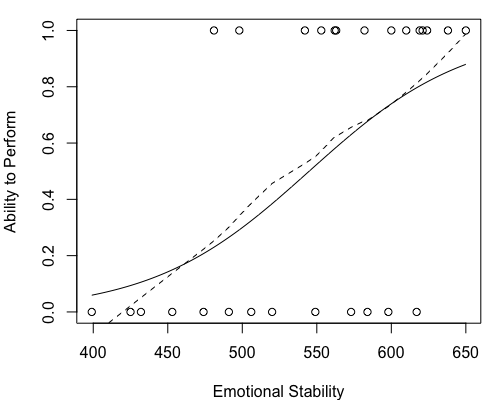
\includegraphics[width=.5\linewidth]{p1/9b.png}
	\end{figure}
	The fitted logistic response function appears to fit well.
	
	\item 
	Obtain $\exp(b_1)$ and interpret this number.
	
	$\exp(b_1) = 1.0191$. The odds ratio $\widehat{OR} = \exp(b_1) = 1.0191$ means that the odds of being able to perform in a task group are estimated to increase by about 1.9 percent with each unit increase in the score of employee's emotional stability.
	
	\item 
	What is the estimated probability that employees with an emotional stability test score of 550 will be able to perform in a task group?
	
	The estimated probability is $\hat{\pi}(550) = \frac{\exp(-10.309 + 0.019\cdot 500)}{1 + \exp(-10.309 + 0.019\cdot 500)} = 0.308$.
	
	\item 
	Estimate the emotional stability test score for which 70 percent of the employees with this test score are expected to be able to perform in a task group.
	
	Solving
	\[
	\log\pa{\frac{0.7}{1-0.7}} = -10.309 + 0.019X
	\]
	we have $X=587$. So with the emotional stability test score being 587, 70 percent of the employees are expected to be able to perform in a task group.
	
	\item 
	Fit a probit mean response function (14.12) to the data. Quantitatively compare the fit here with the logistic fit obtain in part (a). What do you conclude?
	\lstinputlisting{p1/9f.txt}
	The probit mean response function is
	\[
	\hat{\pi} = \Phi(-6.374 + 0.012X)
	\]
	The coefficients of $X$ are close to one another in the two functions, but the intercept is larger in the probit mean response function.
\end{enumerate}

\section*{Problem 2}
(Ex. 14.13) \textbf{Car purchase}
\begin{enumerate}[a.]
	\item 
	Find the maximum likelihood estimates of $\beta_0$, $\beta_1$ and $\beta_2$. State the fitted response function.
	\lstinputlisting{p2/13a.txt}
	The fitted response function is 
	\[
	\hat{\pi} = \frac{\exp(-4.739 + 0.068X_1 + 0.599X_2)}{1 + \exp(-4.739 + 0.068X_1 + 0.599X_2)}
	\]
	The maximum likelihood estimate of $\beta_0$, $\beta_1$ and $\beta_2$ are $b_0 = -4.739$, $b_1 = 0.068$ and $b_2 = 0.599$.
	
	\item 
	Obtain $\exp(b_1)$ and $\exp(b_2)$ and interpret these numbers.
	
	$\exp(b_1) = 1.070079$ and $\exp(b_2) = 1.819627$. The odds ratio $\widehat{OR}_1 = \exp(b_1) = 1.070079$ means that, with the current age of the oldest family automobile($X_2$) fixed, the odds of the family purchasing a new car are estimated to increase by about 7 percent with each unit increase in annual family income($X_1$). The odds ratio $\widehat{OR}_2 = \exp(b_2) = 1.819627$ means that, with the annual family income($X_1$) fixed, the odds of the family purchasing a new car are estimated to increase by about 82 percent with each unit increase in the current age of the oldest family automobile($X_2$).
	
	\item 
	What is the estimated probability that a family with annual income of \$50 thousand and an oldest car of 3 years will purchase a new car next year?
	
	The estimated probability is $\hat{\pi}(50, 3) = \frac{\exp(-4.739 + 0.068\cdot 50 + 0.599\cdot 3)}{1 + \exp(-4.739 + 0.068\cdot 50 + 0.599\cdot 3)} = 0.61254$.
\end{enumerate}

\section*{Problem 3}
(Ex. 14.12) \textbf{Toxicity experiment}
\begin{enumerate}[a.]
	\item 
	Plot the estimated proportions $p_j = Y_{.j} / n_j$ against $X_j$. Does the plot support the analyst's belief that the logistic response function is appropriate?
	\begin{figure}[H]
		\centering
		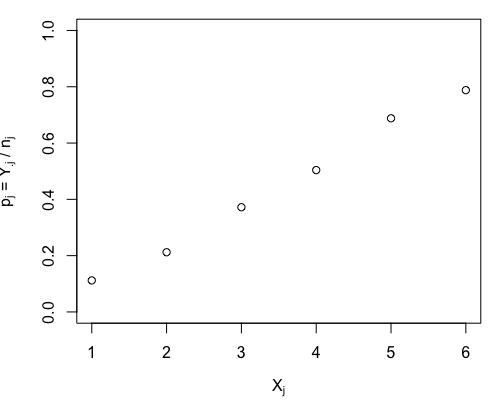
\includegraphics[width=.5\linewidth]{p3/12a.png}
	\end{figure}
	It supports the analyst's belief that the logistic response function is appropriate.
	
	\item 
	Find the maximum likelihood estimates of $\beta_0$ and $\beta_1$. State the fitted response function.
	\lstinputlisting{p3/12b.txt}
	The fitted response function is 
	\[
	\hat{\pi} = \frac{\exp(-2.644 + 0.674X)}{1 + \exp(-2.644 + 0.674X)}
	\]
	The maximum likelihood estimate of $\beta_0$ and $\beta_1$ are $b_0 = -2.644$ and $b_1 = 0.674$.
	
	\item 
	Obtain a scatter plot of the data with the estimated proportions from part (a), and superimpose the fitted logistic response function from part (b). Does the fitted logistic response function appear to fit well?
	\begin{figure}[H]
		\centering
		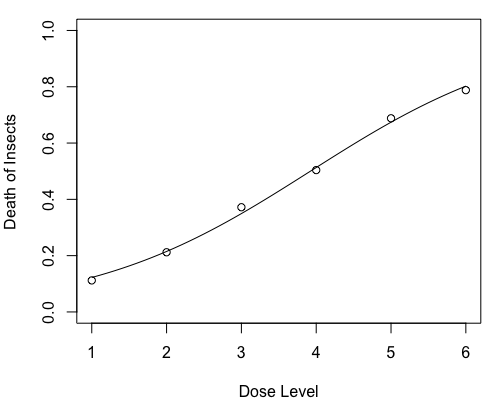
\includegraphics[width=.5\linewidth]{p3/12c.png}
	\end{figure}
	The fitted logistic response function appears to fit well.
	
	\item 
	Obtain $\exp(b_1)$ and interpret this number.
	
	$\exp(b_1) = 1.962056$. The odds ratio $\widehat{OR} = \exp(b_1) = 1.962056$ means that the odds of insects dying due to the toxic substance are estimated to increase by about 96 percent with each unit increase in the dose level.
	
	\item 
	What is the estimated probability that an insect dies when the dose level is $X=3.5$?
	
	The estimated probability is $\hat{\pi}(3.5) = \frac{\exp(-2.644 + 0.674X)}{1 + \exp(-2.644 + 0.674X)} = 0.429$.
	
	\item 
	What is the estimated median lethal dose---that is, the dose for which 50 percent of the experimental insects are expected to die?
	
	Solving
	\[
	\log\pa{\frac{0.5}{1-0.5}} = -2.644 + 0.674X
	\]
	we have $X=3.92$. So with the does level being 3.92, 50 percent of the experimental insects are expected to die.
\end{enumerate}

\end{document}

